\documentclass[border=4pt]{standalone}
\usepackage{amsmath,amssymb}
\usepackage{tikz}
\begin{document}
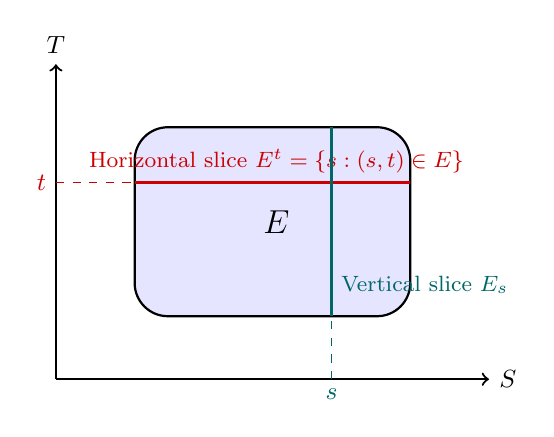
\begin{tikzpicture}[font=\small]
  \draw[->, thick] (0,0) -- (5.5,0) node[right] {$S$};
  \draw[->, thick] (0,0) -- (0,4.0) node[above] {$T$};

  % Set E
  \draw[thick, fill=blue!10, rounded corners=12pt] (1.0, 0.8) rectangle (4.5, 3.2);
  \node at (2.8, 2.0) {\large $E$};

  % Horizontal section
  \draw[very thick, red!80!black] (1.0, 2.5) -- (4.5, 2.5);
  \draw[dashed, red!80!black] (0, 2.5) node[left] {$t$} -- (1.0, 2.5);
  \node[red!80!black, font=\footnotesize, above] at (2.8, 2.5) {Horizontal slice $E^t = \{s : (s,t) \in E\}$};

  % Vertical section
  \draw[very thick, teal!80!black] (3.5, 0.8) -- (3.5, 3.2);
  \draw[dashed, teal!80!black] (3.5, 0) node[below] {$s$} -- (3.5, 0.8);
  \node[teal!80!black, font=\footnotesize, right] at (3.5, 1.2) {Vertical slice $E_s$};
\end{tikzpicture}
\end{document}